\documentclass[12pt]{article} % Enforces the minimum 12-point font requirement

% --- Packages for Formatting and Styling ---
\usepackage{mathptmx} % Sets font to Times Roman to meet font guidelines
\usepackage{setspace}
\singlespacing % Enforces single-spaced text requirement
\usepackage[margin=1in]{geometry}
\usepackage{fancyhdr} % Allows creation of the mandatory running header
\usepackage{graphicx} % Essential for importing and formatting figures
\usepackage{amsmath}  % Essential for mathematical equations and arrays
\usepackage{booktabs}
\usepackage[super, comma, sort&compress]{natbib} % Configures AIP superscript citations
\usepackage{xcolor}
\graphicspath{{figures/}}

% --- Header Configuration ---
\pagestyle{fancy}
\fancyhf{}
\renewcommand{\headrulewidth}{0pt} % Removes the horizontal line under the header
\fancyhead[R]{Jonathan Fuentes Rosales | Mentor: John Brewer} % Mandatory SULI header
\fancyfoot[C]{\thepage} % Centers page number at the bottom

% --- AIP Section Heading Configuration ---
\usepackage{titlesec}
\titleformat{\section}{\large\bfseries\MakeUppercase}{\Roman{section}.}{1em}{}
\titleformat{\subsection}{\normalsize\bfseries}{\Alph{subsection}.}{1em}{}
\titleformat{\subsubsection}{\normalsize\itshape}{\arabic{subsubsection}.}{1em}{}
\titleformat{\paragraph}[runin]{\normalsize\itshape}{\alph{paragraph}.}{1em}{}

% ============================================================================
% ACTION REQUIRED BEFORE SUBMISSION -- 3 items, each printed in RED in the PDF
% so they cannot be missed:
%   1. The disclaimer clause (mandatory, not supplied with the guidelines).
%   2. Related activities and publications (personal record, not in the repo).
%   3. Acknowledgments -- confirm programmatic support wording.
% ============================================================================
\newcommand{\TODO}[1]{\textcolor{red}{\textbf{[#1]}}}

\begin{document}

% --- Technical Abstract ---
\begin{center}
    \textbf{ABSTRACT}
\end{center}
\begin{quote}
Regional transmission organizations must match electricity supply and demand
continuously, and day-ahead demand forecasts are least reliable exactly when the
consequences of error are greatest. This project evaluated whether Adaptive
Conditional Neural Processes (AdaCNP), a probabilistic few-shot method reported
to improve extreme-load forecasting on the PJM and ISO-NE systems, reproduces
that advantage on ERCOT data. A leave-one-event-out protocol was built over 17
load-eligible extreme cold events spanning 2002--2026, with plus/minus seven-day
buffers excluded from both training and context retrieval, a 09:00 CT day-ahead
issuance cutoff enforced throughout, and an adopted treatment for hours whose
load-shed status is documented or unknown. The comparison against a standard
Conditional Neural Process baseline was pre-registered: the analysis plan,
primary endpoint, statistical test and decision rule were committed to version
control before any confirmatory run executed. Two findings emerged. First, and
most consequential for grid operations, both models are severely overconfident
during extreme events. The nominal 90 percent prediction interval contains the
observed load for 96 percent of normal-period hours but only 63 percent of
held-out extreme-event hours, and coverage degrades further as events become more
severe. The failure is directional: the models systematically under-forecast
demand while reporting high confidence. Second, the pre-registered test detected
an AdaCNP advantage on the primary metric, a mean paired difference of 0.459 in
Gaussian negative log likelihood with 95 percent confidence interval 0.108 to
0.811 and p equal to 0.014 over 17 events. Three qualifications are reported
alongside it: the observed effect lies just below the study's minimum detectable
effect of 0.495, so power at the realised effect size was approximately 77
percent; the advantage appears only in the pre-registered configuration; and the
design cannot resolve an effect of the magnitude the source paper reports, which
is roughly an order of magnitude smaller. A measurement of the proposed mechanism
found that AdaCNP places less weight on cold historical analogues than uniform
weighting does, so the performance gain is not explained by the mechanism its
authors describe. The calibration deficit, rather than the architecture
comparison, is the result most relevant to reserve planning and early generation
commitment.
\end{quote}

\vspace{1em}
\noindent\textbf{DISCLAIMER}\\[0.3em]
\small This project was supported in part by the U.S. Department of Energy, Office of Science, Office of Workforce Development for Teachers and Scientists (WDTS), under the Science Undergraduate Laboratory Internships (SULI) Program through an appointment at the National Energy Technology Laboratory (NETL). Neither the United States Government nor any agency thereof, nor any of its employees, nor the support contractor, nor any of their employees, makes any warranty, express or implied, or assumes any legal liability or responsibility for the accuracy, completeness, or usefulness of any information, apparatus, product, or process disclosed, or represents that its use would not infringe privately owned rights. Reference herein to any specific commercial product, process, or service by trade name, trademark, manufacturer, or otherwise does not necessarily constitute or imply its endorsement, recommendation, or favoring by the United States Government or any agency thereof. The views and opinions of authors expressed herein do not necessarily state or reflect those of the United States Government or any agency thereof.” Motivation Why accurate energy forecasting matters to the DOE mission • [Frame the problem: what decision depends on an energy forecast, and at what scale?] • [Who relies on it — grid operators, resource planners, DOE program offices?] • [What is the cost of being wrong: reliability, dollars, emissions?] • [One anchoring statistic or short real-world example] • [Connect explicitly to NETL / DOE mission relevance] 3 Background: Conventional Forecasting and Its Limits Where existing approaches fall short Current state of practice • [Name the standard methods used today — statistical, physics-based, or ML] • [What assumptions do they rely on?] Known limitations • [Limitation 1 — e.g. accuracy under volatile or extreme conditions] • [Limitation 2 — e.g. data requirements, computational cost, interpretability] • [The specific gap your project addresses] 4 Research Objectives The specific question this project set out to answer Research question • [State the question in one sentence a non-specialist could follow] Objectives 1. [Objective 1 — what you built, measured, or tested] 2. [Objective 2 — how you evaluated it] 3. [Objective 3 — what you compared it against] Scope • [What was in scope for a 10-week internship, and what was not] 5 Data and Methods What went in, what was used, and how it was evaluated Data Novel method • [Source(s) and provider] • [Name the method] • [Time span and resolution] • [What makes it novel here] • [Number of records / features] • • [Cleaning and preprocessing steps] [Key hyperparameters or settings] • [Software and compute used] Evaluation • [Baseline model(s) for comparison] • [Metrics: e.g. RMSE, MAE, MAPE] • [Train / validation / test split] • [Validation strategy] 6 Approach End-to-end workflow from raw data to validated forecast Workflow Workflow diagram 1. [Acquire and clean input data] 2. [Engineer features / define inputs] 3. [Train the model] [ Insert your pipeline or architecture diagram here — a single clear figure is worth more than a list ] 4. [Tune and validate] 5. [Benchmark against baseline] 6. [Interpret and report] 7 Results I: Forecast Accuracy vs. Baseline PLACEHOLDER DATA — replace with your measured results Forecast Error by Horizon (lower is better) Baseline method Novel method 16 14.1 14 MAPE (\%) 12 9.5 10 8 6 4 6.8 4.2 9.4 6.2 4.6 3.1 2 0 1-hour 6-hour 24-hour 7-day Forecast horizon 8 Results II: Predicted vs. Observed Demand PLACEHOLDER DATA — replace with your measured results Predicted vs. Observed Load, Representative Day Observed Novel method forecast Baseline forecast 04:00 08:00 16:00 900 800 Load (MW) 700 600 500 400 300 200 100 0 00:00 12:00 Hour of day 20:00 24:00 9 Discussion What the results mean — and what they do not Interpretation • [Why does the novel method outperform / underperform?] • [Which conditions drive the largest gains?] • [How do results compare to published work?] • [Practical significance for a grid operator or planner] Limitations • [Data coverage or quality constraints] • [Assumptions that may not generalize] • [Computational or runtime trade-offs] • [What a longer study would need to confirm] 10 Conclusions and Future Work Key takeaways from the summer and where the work goes next Key findings Impact [Finding 1 — the headline result, quantified] • • [Finding 2] • [Who could use it and how] • [Finding 3] • [Broader mission relevance] • [What this enables for DOE / NETL] Future work • [Next experiment or dataset] • [Model refinement to pursue] • [Path to publication or deployment] 11 Acknowledgments Thank you — questions welcome With thanks to • [Mentor name] — NETL, for project guidance and mentorship • [Federal team supervisor / division director name] • [Colleagues, group members, or collaborators who contributed] Support • This work was supported in part by the U.S. Department of Energy, Office of Science, Office of Workforce Development for Teachers and Scientists (WDTS), under the Science Undergraduate Laboratory Internships (SULI) program. Questions? [your.email@example.edu] 12 13 14 www.NETL.DOE.gov @NETL\_DOE @NETL\_DOE @NationalEnergyTechnologyLaboratory CONTACT:
\normalsize

\vspace{1em}

% --- MAIN BODY TEXT ---
% CONSTRAINT: Main text word count must be 1,500 - 3,000 words (SULI).

\section{Introduction}

Electricity cannot be stored economically at grid scale, so a balancing authority
must match generation to demand continuously. That obligation forces a decision
under uncertainty every day: commit generating resources today for demand that
will materialise tomorrow. Under-commit and reserves fall short; over-commit and
consumers pay for capacity that idles. Regional transmission organizations and
independent system operators are permitted to commit resources early, before the
day-ahead market, in order to hedge extreme weather, but doing so runs against
their mandate to dispatch at least cost. The value of that hedge depends entirely
on whether the forecast's stated uncertainty can be trusted.

Extreme weather is where this is hardest and where it matters most. The February
2021 winter storm drove ERCOT to shed firm load. Such events are also rare by
construction, which creates a data problem: a model may have tens of thousands of
ordinary days to learn from and only a handful of the days that actually
determine reserve adequacy. Worse, the relationship between weather and demand is
not stable across regimes, so ordinary days can actively mislead.

This project addressed that problem by testing a published method on new data. Hu
\emph{et al.}\cite{hu2026resilient} propose Adaptive Conditional Neural Processes,
which extend Conditional Neural Processes by weighting historical context
examples according to their similarity to the current forecast target rather than
averaging them uniformly. They report improved extreme-load forecasting on the
PJM and ISO-NE systems. The goal of this project was to determine whether that
reported advantage reproduces on ERCOT data, and to establish what such a test
can and cannot demonstrate given the number of extreme events ERCOT's history
supplies.

Project boundaries were fixed at the outset. The comparison is AdaCNP against
standard CNP only, on a shared encoder--decoder backbone, with the aggregation
mechanism as the single intended difference; no other architectures were
evaluated. Evaluation is restricted to held-out extreme cold events under a
leave-one-event-out protocol. All work is retrospective on historical data;
nothing was deployed operationally.

\section{Methodology}

\subsection{Data and event definition}

The target series is hourly ERCOT system load from 2002 to 2026, adopted by
content hash rather than by filename so that provenance is exact. Extreme events
come from a frozen inventory derived from a regional temperature index, with
severity characterised by cold margin in degrees Celsius. Seventeen events are
load-eligible, meaning they fall within the span of the load record; this count
is derived from the artifacts at run time rather than hard-coded, so the protocol
adapts if the inventory changes.

An episode targets one calendar day and predicts its 24-hour load vector. Inputs
are calendar terms, the 24 most recent complete hourly load observations, the 24
most recent temperature observations, the 24-hour rolling mean temperature at the
cutoff, and non-linear heating and cooling terms: 57 features in total. Every
feature is restricted to information complete at or before the day-ahead issuance
instant, fixed at 09:00 America/Chicago on the day preceding the target day.

\subsection{Leakage control and censored observations}

Three protections were built and verified by automated test rather than by
inspection. Outer partitions are leave-one-event-out with a seven-day buffer on
each side of the held-out event, excluded from both training and context
retrieval. Both model arms consume a single persisted context-index file, re-read
from disk by each arm, so their context sets are byte-identical by construction.
Normalization statistics are fitted on each fold's training partition only.

Load measured during directed load shed is a lower bound on the demand that would
otherwise have materialised, not an observation of it. Across the 1{,}271
event-hours in the record, 80 hours are documented as shed, zero hours are
documented as not shed, and the remaining 1{,}191 carry no primary-source
determination either way. The adopted treatment excludes documented shed hours
from the primary metric, retains undetermined hours while flagging them, and
reports an all-hours served-load likelihood as a secondary diagnostic on a
different estimand. Resolving the undetermined hours in either direction would
assert a finding the record does not support.

\subsection{Statistical design and pre-registration}

The primary metric is Gaussian negative log likelihood on held-out event-period
load. Because normalization is fitted per fold, likelihood values are not
comparable across folds; the only admissible quantity is the within-event paired
difference between arms, which share a fold's normalizer and context file. The
unit of analysis is therefore one paired difference per event with the three
frozen seeds averaged, giving a sample size of 17.

The analysis was pre-registered. The primary endpoint, the configuration to be
tested, the statistical test, the significance level, the robustness checks and
the decision rule, including what a null result would be permitted to claim, were
committed to version control before any confirmatory run executed. The analysis
code was committed at the same time and validated against earlier exploratory
data, so the reported number was produced by code whose commit provably predates
the data it analysed. The tested configuration was chosen for fidelity to Hu
\emph{et al.}---temperature features and randomly sampled context sets, matching
their inputs and their sampling procedure---and explicitly not for the size of
effect it had shown in exploratory work.

A power analysis preceded the confirmatory runs, using variance measured from
exploratory data rather than assumed. It established the minimum detectable
effect at 80 percent power, reported alongside every result so that a null can be
distinguished from an absence of power.

The full sweep comprised 408 runs---17 folds by 2 arms by 2 feature sets by 2
context conditions by 3 seeds---executed on CPU with zero failures. Training
length was not fixed by hand: each run trained to a ceiling and the reported
parameters were those achieving the best inner-validation likelihood, with inner
validation drawn from the fold's own training partition. Selecting on the
held-out event would have constituted leakage.

\section{Results and Discussion}

\subsection{Calibration fails during extreme events, in the dangerous direction}

The most operationally consequential result is not the comparison between
architectures. It is that both models' stated uncertainty is untrustworthy
precisely in the regime the project set out to study.

\begin{figure}[htbp]
\centering
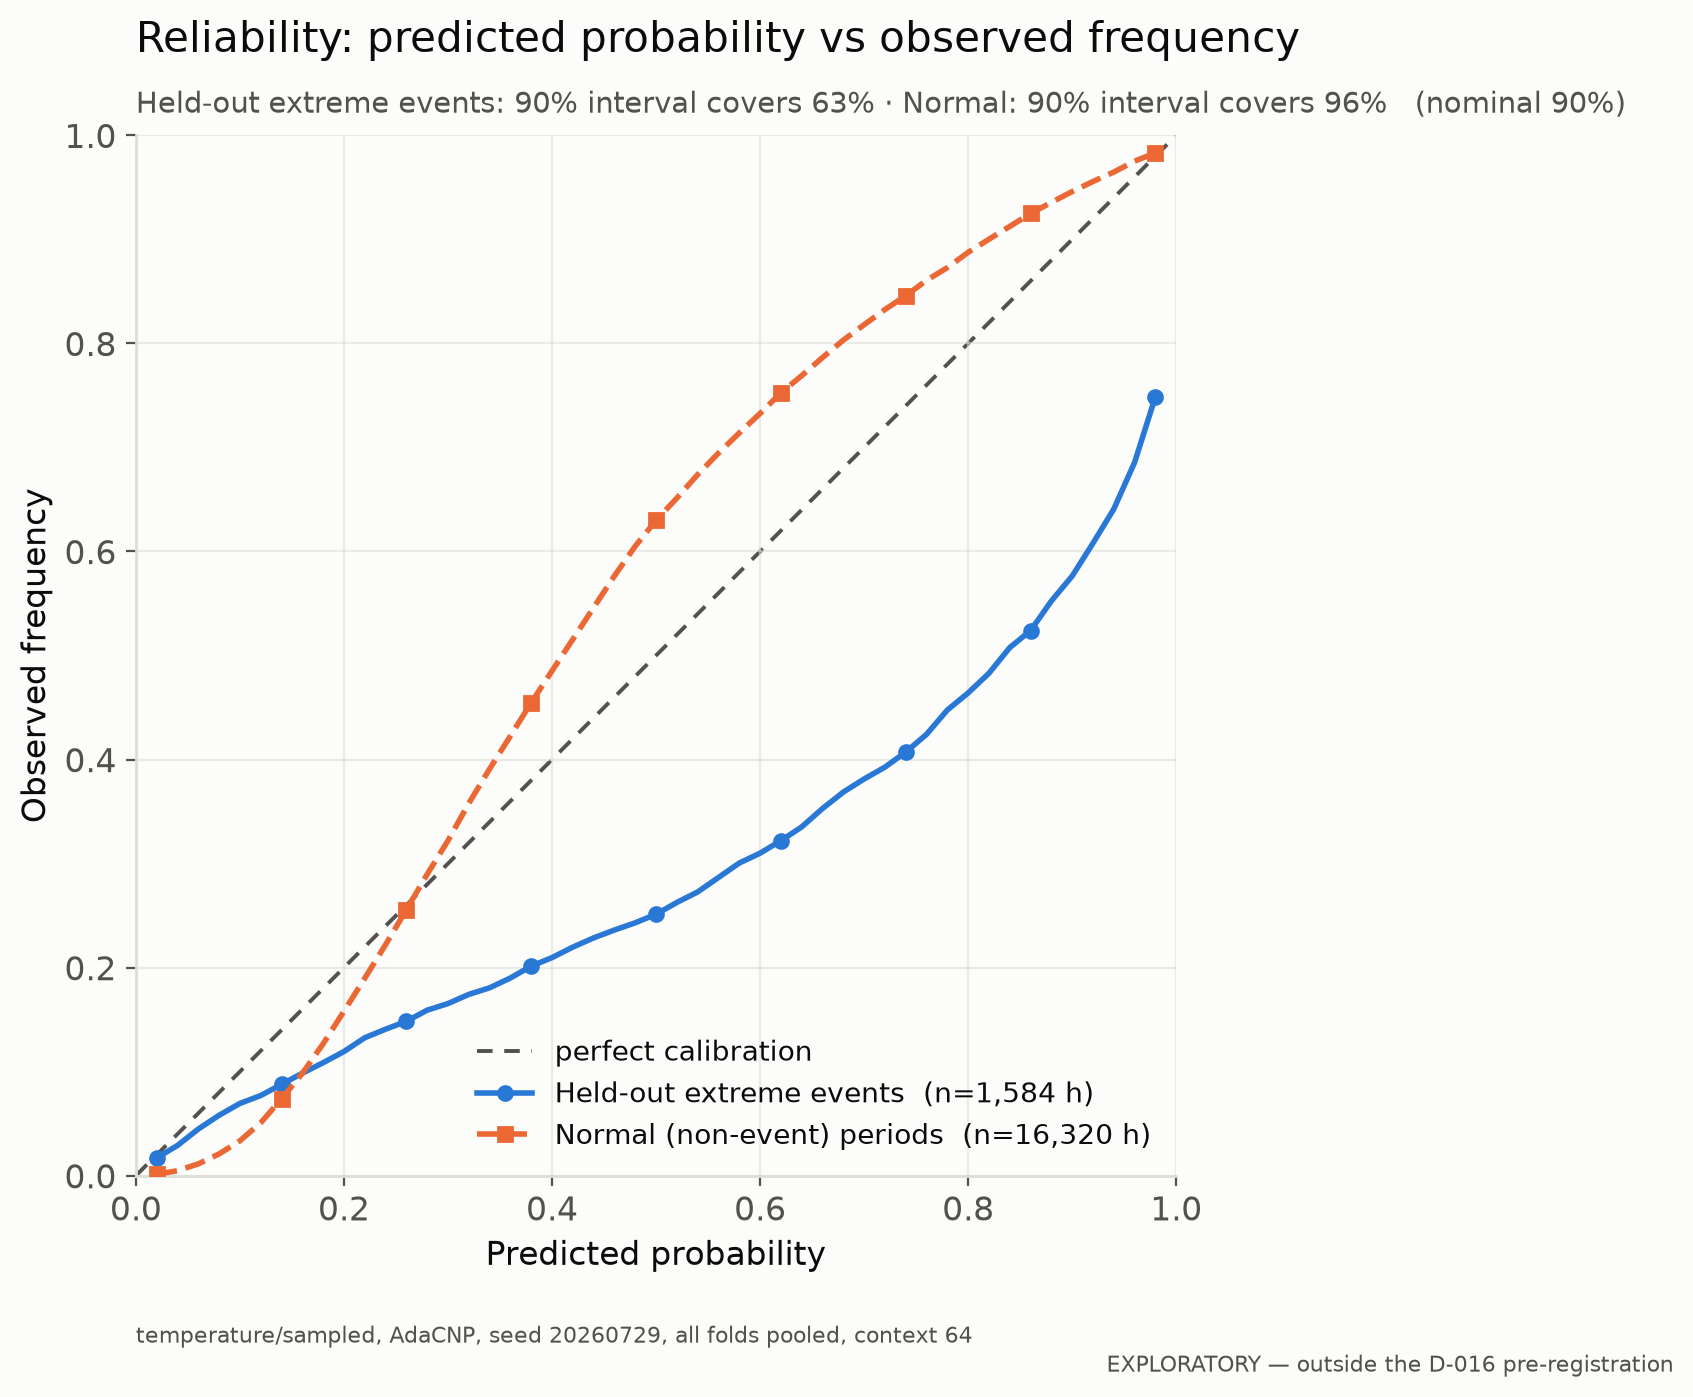
\includegraphics[width=0.66\textwidth]{fig1_reliability.png}
\caption{Reliability of the predictive distribution, by regime. For each nominal
probability the model's corresponding quantile is computed and the observed
frequency of outcomes at or below it is plotted; a perfectly calibrated forecast
follows the diagonal. Both curves come from the same trained models, evaluated on
held-out extreme-event days and on non-event days drawn from the same folds'
inner-validation blocks. The 90 percent central interval contains the observed
load for 96 percent of normal-period hours but only 63 percent of extreme-event
hours. \textbf{Exploratory: outside the pre-registered analysis.}}
\label{fig:reliability}
\end{figure}

Figure~\ref{fig:reliability} shows the failure. In normal conditions the forecast
is honest and slightly conservative, its intervals marginally too wide, which is
the safe direction in which to err. During held-out extreme events the same
models' 90 percent interval covers 63 percent of hours. The extreme-event curve
also lies below the diagonal across its entire range, meaning fewer outcomes fall
below each predicted quantile than the model expects: the models systematically
under-forecast demand during extreme cold while reporting high confidence. This
is the error mode that would lead an operator to skip an expensive early
commitment.

\begin{figure}[htbp]
\centering
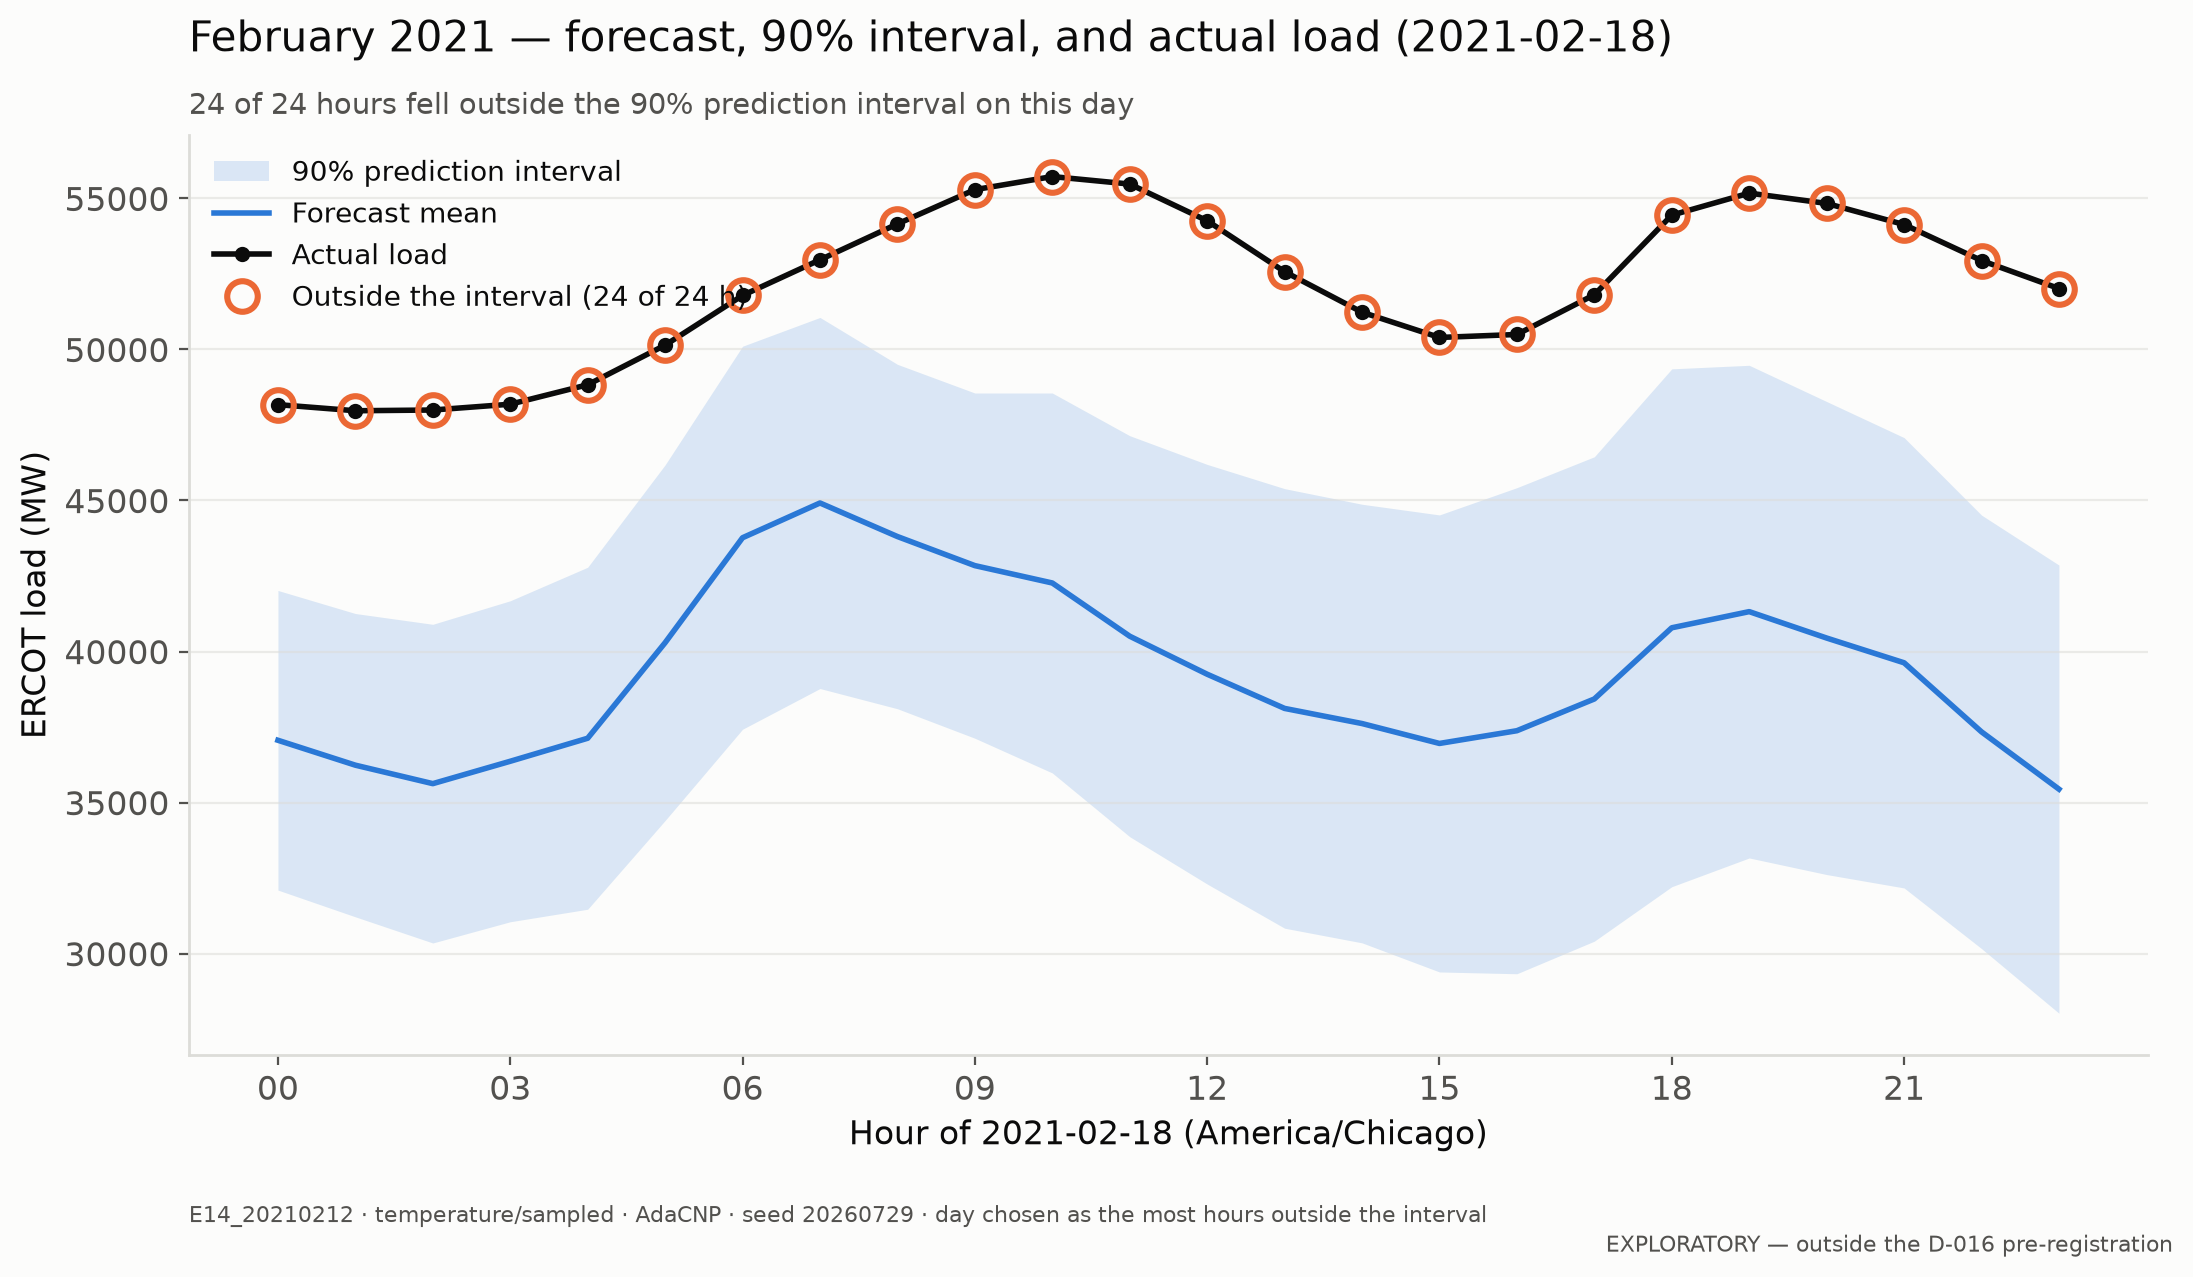
\includegraphics[width=0.82\textwidth]{fig2_february_2021.png}
\caption{A single day of the February 2021 event. The day shown was selected by a
stated rule---the day of that event with the most hours falling outside the 90
percent interval---and is therefore the worst case, not a typical day. All 24
hours fell outside the interval, with observed load running roughly 10 GW above
the forecast mean. The day carries no documented load-shed hours, so the gap
reflects forecast error rather than curtailed demand. \textbf{Exploratory.}}
\label{fig:feb2021}
\end{figure}

Figure~\ref{fig:feb2021} makes the magnitude concrete for one day of the February
2021 event. Figure~\ref{fig:severity} shows that the deficit is not uniform:
coverage declines as events become more severe, at approximately $-0.037$ per
degree Celsius of cold margin for CNP ($r=-0.55$) and $-0.031$ for AdaCNP
($r=-0.51$). Only the mildest events approach nominal coverage. For practice, the
implication is that calibration is worst exactly where reserve margins are
thinnest.

\begin{figure}[htbp]
\centering
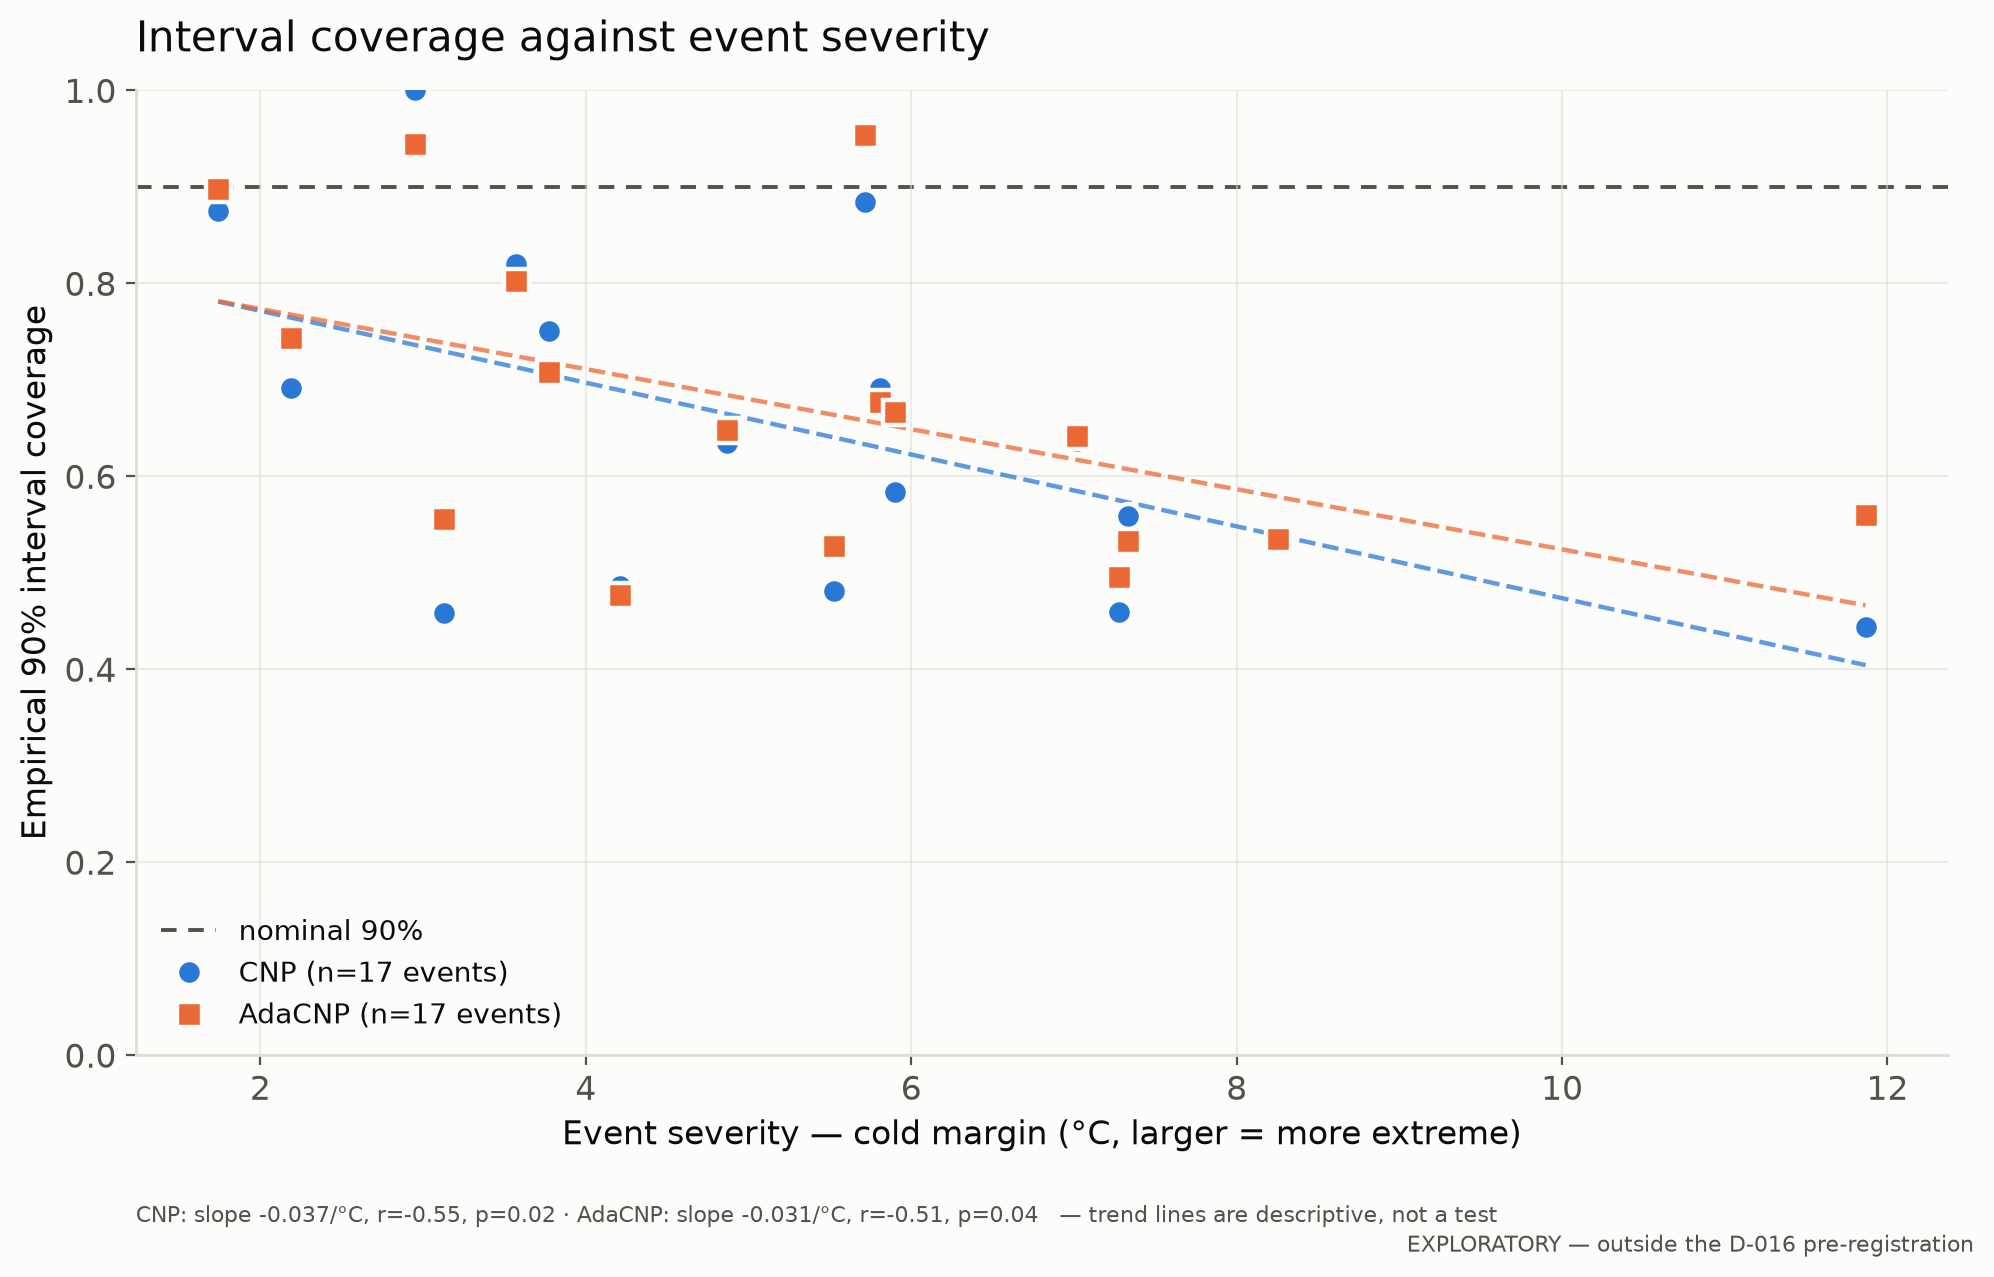
\includegraphics[width=0.74\textwidth]{fig3_coverage_vs_severity.png}
\caption{Empirical 90 percent interval coverage against event severity across all
17 leave-one-event-out folds, both arms. Trend lines are descriptive and form no
part of the pre-registered analysis. \textbf{Exploratory.}}
\label{fig:severity}
\end{figure}

\subsection{The pre-registered comparison}

The pre-registered test detected an advantage for AdaCNP on held-out ERCOT
extreme events; Table~\ref{tab:primary} reports it.

\begin{table}[htbp]
\centering
\caption{Pre-registered primary result. Positive differences favour AdaCNP.}
\label{tab:primary}
\begin{tabular}{lr}
\toprule
Quantity & Value \\
\midrule
Events ($n$) & 17 \\
Seeds per event & 3 \\
Mean paired difference & $+0.459$ \\
95\% confidence interval & $[+0.108,\ +0.811]$ \\
Two-sided paired $t$-test & $p = 0.014$ \\
Wilcoxon signed-rank (robustness) & $p = 0.020$ \\
Minimum detectable effect & $0.495$ \\
\bottomrule
\end{tabular}
\end{table}

Predeclared robustness checks are consistent. The Wilcoxon signed-rank test
agrees with the $t$-test, so the pre-registered inconclusive branch was not
triggered. Excluding the one fold reduced to a single held-out day gives a mean
of $+0.486$ ($p=0.014$). A leave-one-fold-out jackknife spans $[+0.343,+0.501]$
with the sign stable across all 17 refits, so no single event drives the finding,
and 11 of 17 events favour AdaCNP. Secondary metrics point the same way:
continuous ranked probability score 0.469 against 0.486, root mean squared error
0.756 against 0.773, and calibration error 0.247 against 0.272. The frozen
protocol reserves adjudication to the primary metric, so these are reported for
interpretation only.

\begin{figure}[htbp]
\centering
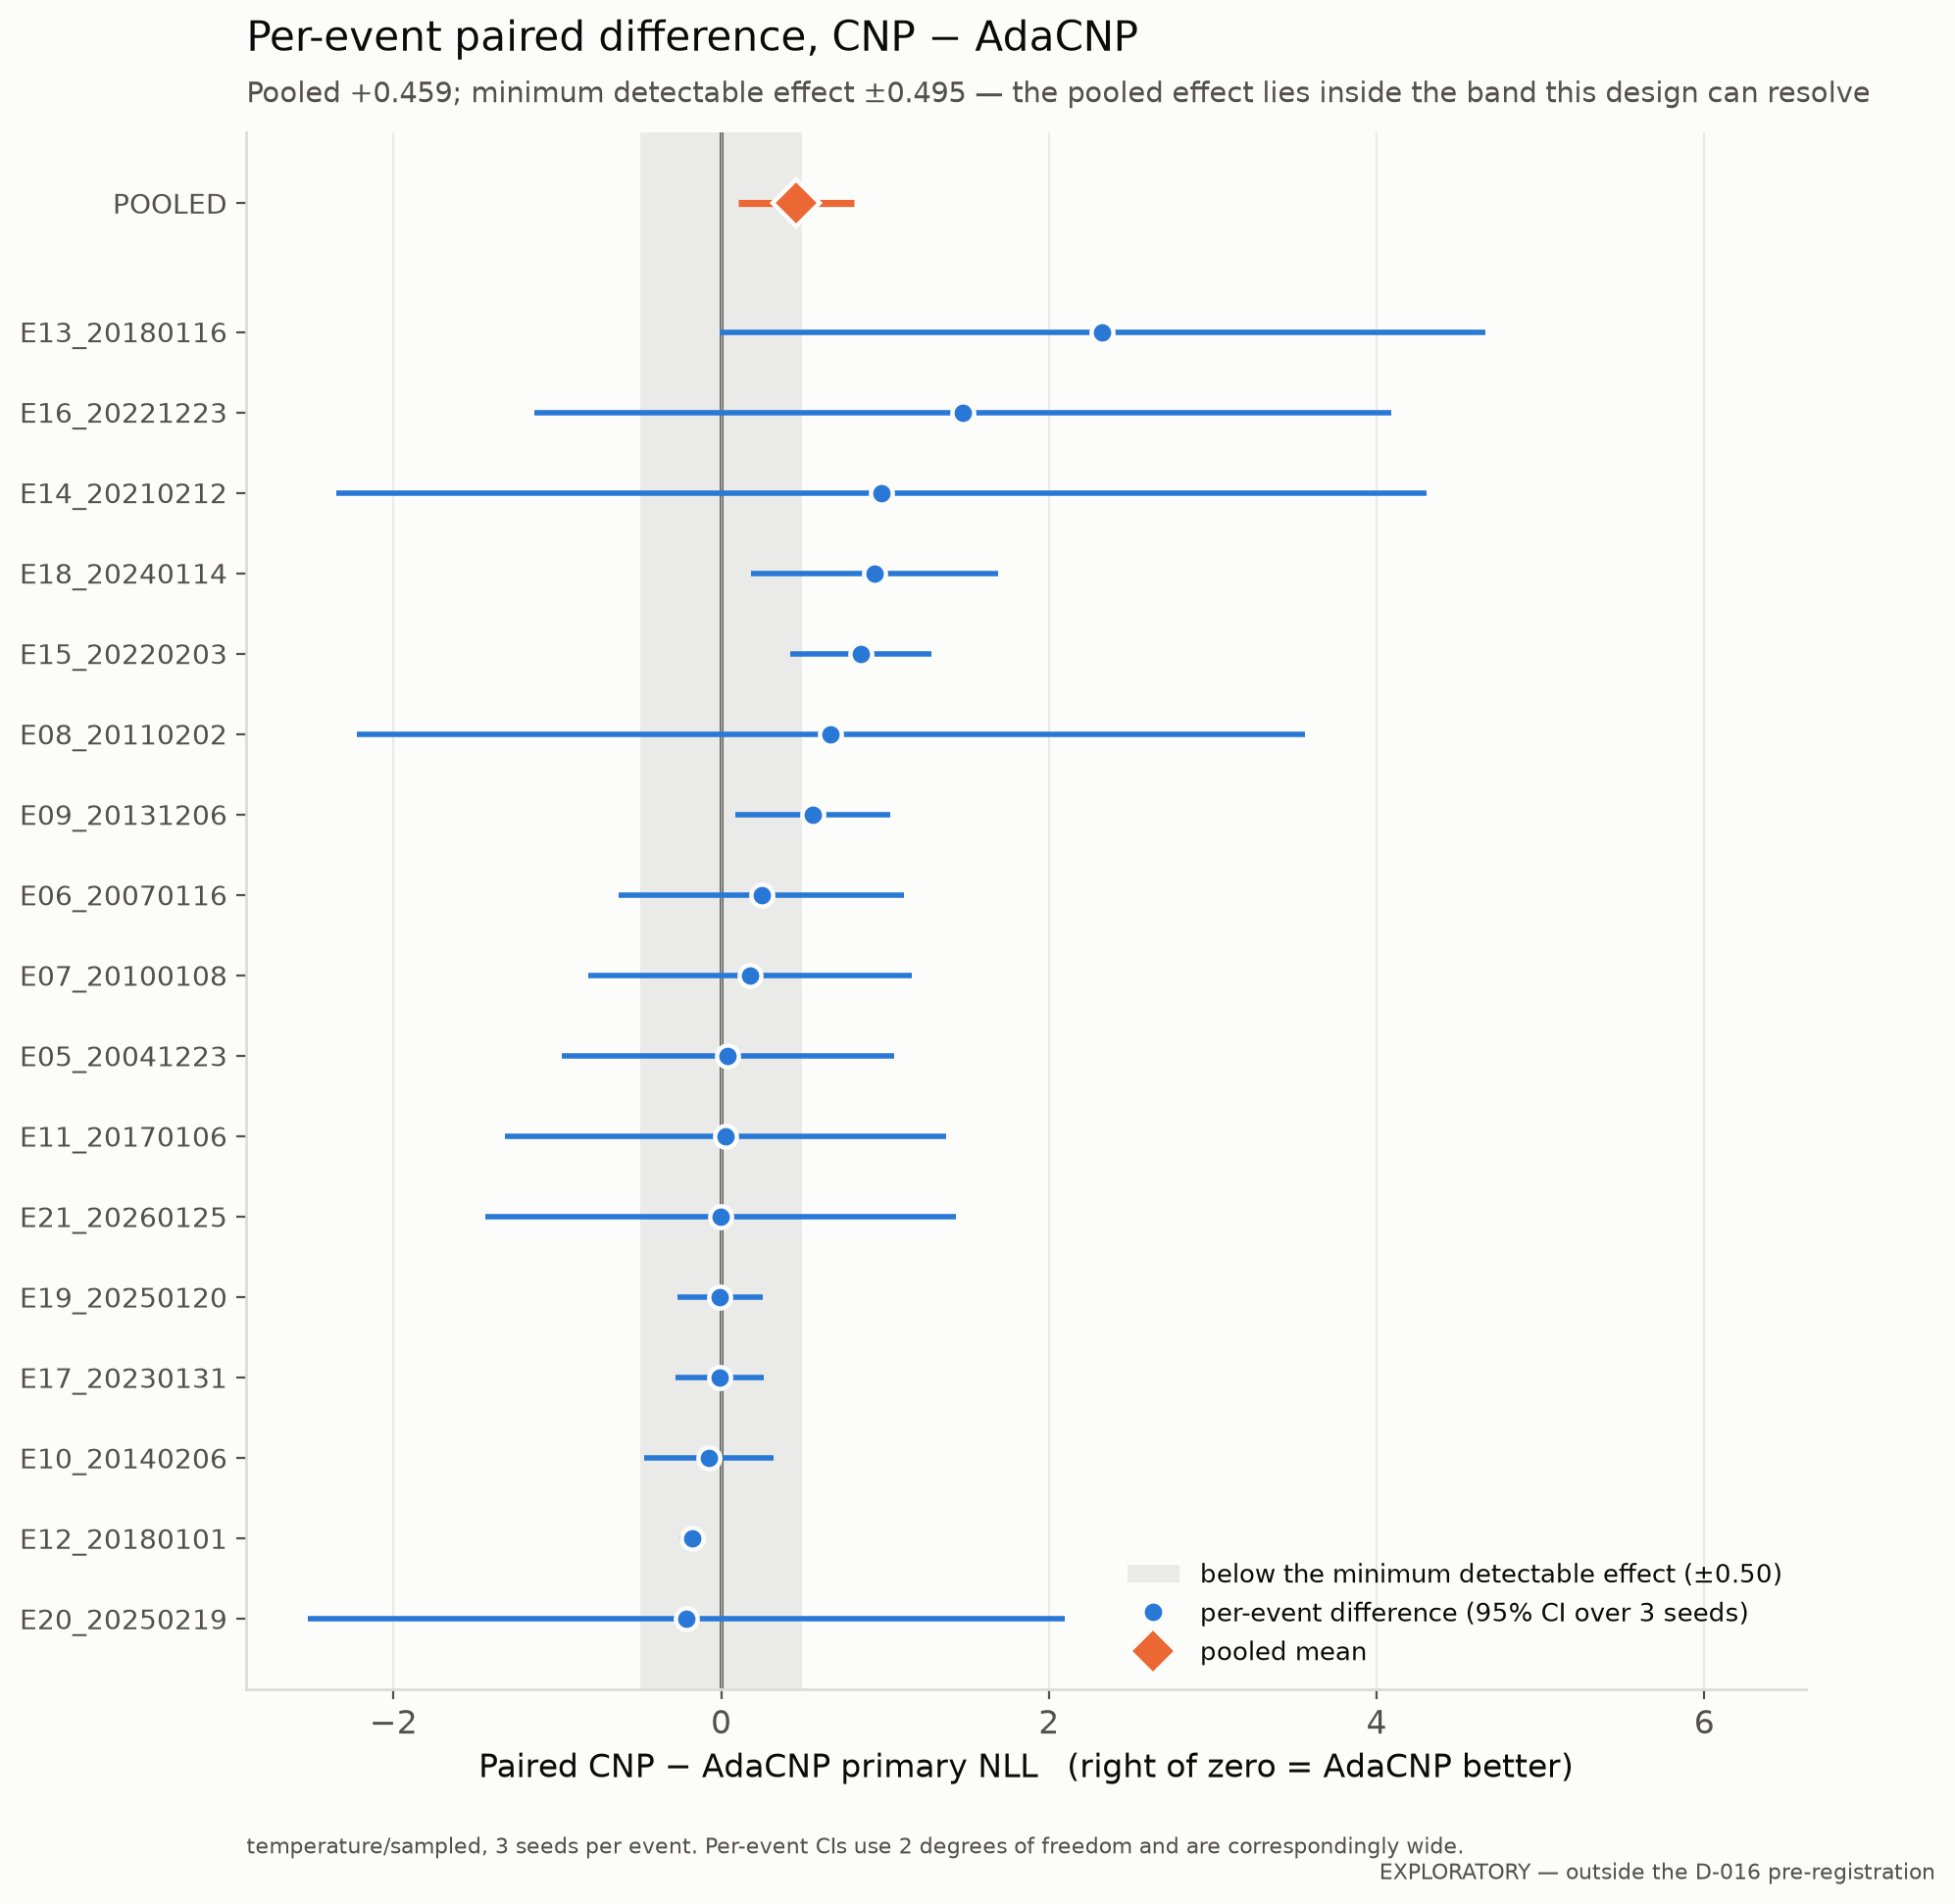
\includegraphics[width=0.76\textwidth]{fig4_forest.png}
\caption{Per-event paired differences with 95 percent confidence intervals, the
pooled mean, and the shaded band below the minimum detectable effect. Per-event
intervals use two degrees of freedom and are correspondingly wide; they indicate
shape, not per-event significance. \textbf{Exploratory presentation of the
pre-registered quantity; the confirmatory result is Table~\ref{tab:primary}.}}
\label{fig:forest}
\end{figure}

Three qualifications belong with that result rather than in a footnote.

First, the observed effect of $+0.459$ lies just below the minimum detectable
effect of $0.495$. The study therefore had roughly 77 percent power at the effect
size it actually found, short of the 80 percent target. The result satisfies the
pre-registered decision rule, but it sits near the edge of what this design can
resolve and warrants independent replication rather than treatment as settled.

Second, the advantage appears only in the pre-registered configuration. Of the
four configurations run, the pre-registered one gave $+0.459$; the same feature
set with nearest-neighbour context retrieval gave $-0.240$, favouring the
baseline. Had the configuration been chosen after inspecting results, a range of
conclusions could have been supported. The pre-registration is what makes the
reported claim admissible, and that dependence is stated deliberately.

Third, this is not a measurement of the effect size Hu \emph{et al.} report.
Their AdaCNP-over-CNP likelihood margin corresponds to roughly 0.02 to 0.12 in
the units used here, an order of magnitude below this design's minimum detectable
effect. The power analysis puts this study's power to detect a margin that size
at 5 to 9 percent and estimates that several hundred events would be required;
ERCOT's history supplies 17. A null would consequently have been uninformative
about the source finding, which is precisely why the minimum detectable effect is
reported beside the estimate.

\subsection{The mechanism does not behave as described}

AdaCNP's proposed advantage comes from concentrating attention on relevant
historical analogues, and during extreme cold that means similarly cold days.
This is directly measurable once temperature features are present. Under uniform
weighting, CNP places 0.105 of its context weight on cold days, which is simply
the cold fraction of its context set. AdaCNP places 0.079: it de-emphasises cold
analogues, and its weighting is only mildly non-uniform, using 57.5 effective
context points out of 64.

AdaCNP therefore scores better on held-out extreme events, but not by doing what
its authors describe. Whatever produces the improvement observed here, it is not
concentration on cold analogue days. This is an open question and, for future
work, a more interesting one than the score difference itself.

\subsection{Limitations}

The event count is fixed at 17 by ERCOT's history and by the extreme-weather
framing; the power analysis identifies it as the binding constraint. Of the
1{,}584 held-out hours scored per seed, 1{,}139 carry undetermined load-shed
status, so the primary metric carries an unknown amount of censoring
contamination that the record cannot resolve. No day-ahead forecast weather
product with historical issuance timestamps was available, so all temperature
features are past-observed; Hu \emph{et al.} additionally use next-day forecast
temperature, and this remains the largest divergence from their protocol. Three
seeds were used, initialisation noise dominates the measurement, and additional
seeds would be the cheapest available improvement to precision. Finally, only the
primary endpoint is confirmatory; the calibration results and the mechanism
measurement are exploratory and labelled as such throughout.

\section{Conclusions}

The pre-registered comparison detected an advantage for AdaCNP over a standard
CNP baseline on held-out ERCOT extreme cold events: $+0.459$ in Gaussian negative
log likelihood, 95 percent confidence interval $[+0.108,+0.811]$, $p=0.014$,
$n=17$, with robustness checks consistent and no single event driving the result.
The advantage is real by criteria fixed in advance, but it sits near the
resolution limit of the design, it depends on the pre-registered configuration,
and it is not a measurement of the effect size reported in the source work.

The more consequential finding for grid operations is that both models are badly
and directionally overconfident during extreme events. A nominal 90 percent
interval that contains the outcome 96 percent of the time in normal conditions
contains it 63 percent of the time during extreme cold, with the deficit widening
as events worsen. For a balancing authority weighing early generation commitment,
a forecast that is uncertain and says so is manageable; a forecast that is wrong
and confident is not. On this evidence, improving calibration in the extreme
regime would repay more than further architecture comparison.

\subsection{Summary of appointment activities}

Over the appointment I built a complete and reproducible experimental pipeline
for probabilistic extreme-load forecasting on ERCOT data: verified data import
with content-hash provenance, leakage-controlled leave-one-event-out partitioning
with issuance-time enforcement, an adopted treatment for censored load
observations, a CPU-based training and evaluation harness for both model arms, a
pre-registered statistical analysis, and a power analysis quantifying the
design's resolution. Activities included a literature review that identified the
source method, reconstruction and hash verification of the project's inherited
data corpus, a documented audit comparing this implementation against the source
publication, and execution of a 408-run confirmatory sweep. Decisions of record
are captured in a versioned decision log, and every reported figure is
regenerated from committed artifacts by script rather than transcribed.

\subsection{Related activities and publications}

\TODO{TO BE COMPLETED BY AUTHOR. NETL requires a summary of related activities
(presentations, training, conferences, learning activities) and any publications.
This is personal record and is not contained in the project repository. List the
end-of-summer presentation, any training completed, any conferences or seminars
attended, and any publications --- or state ``None.''}

\section*{Acknowledgments}

I thank my mentor, John Brewer, for guidance throughout this appointment, and my
federal team supervisor, Luciane Cunha, for review and support. This work was supported by the
U.S.\ Department of Energy, Office of Science, Science Undergraduate Laboratory
Internship (SULI) program, and was carried out at the National Energy Technology
Laboratory. \TODO{Add any other individuals who directly assisted, if applicable.}

% --- References ---
\bibliographystyle{unsrtnat}
\bibliography{references}

\end{document}
